\documentclass{standalone}
%<--------------------------------------------------------------------------->%
%%% Math %%%
\usepackage{amsmath,amssymb}
\usepackage{mathrsfs,gensymb}
\usepackage{mathtools}
% \usepackage{centernot}
% \usepackage{accents}
% \usepackage[makeroom]{cancel}
% \newcommand{\two}[2]{\substack{ \text{#1} \\ \text{#2} }}
% \newcommand{\raum}{\phantom{=}{\:\,}}
% \newcommand{\st}{s.t.\ }
% \newcommand{\asDemonstrated}{\null\nobreak\hfill\ensuremath{\blacksquare}}
%-----------------------------------------------------------------------------%
%%% TikZ %%%
\usepackage{tikz}
\usetikzlibrary{calc}
% \usetikzlibrary{angles,quotes}
% \usetikzlibrary{intersections,topaths}
% \usetikzlibrary{decorations.markings}
%<--------------------------------------------------------------------------->%

\begin{document}

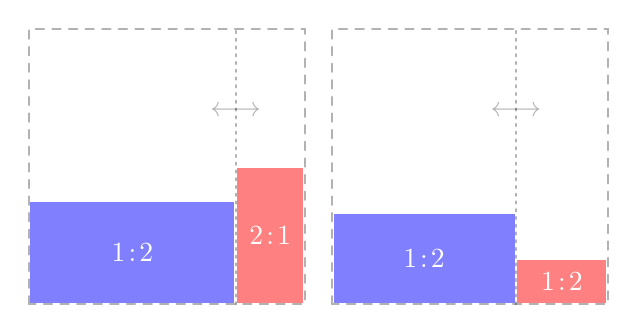
\begin{tikzpicture}[scale=3.5,thick,line cap=round]
	\tikzstyle{jiao}=[solid,circle,draw,fill=white,inner sep=.8pt];
	\tikzstyle{tile1}=[line width=0.1em,draw=white,fill=blue!50];
\tikzstyle{tile2}=[line width=0.1em,draw=white,fill=red!50];
\tikzstyle{tile3}=[line width=0.1em,draw=white,fill=blue!50!red!60];
\tikzstyle{tile4}=[line width=0.1em,draw=white,fill=blue!20!red!60];

	\draw[tile1] (0,0)   rectangle (3/4,3/8);
	\node[white] at ($(0,0)!0.5!(3/4,3/8)$) {$1\!:\!2$};
	\draw[tile2] (3/4,0) rectangle (1,1/2);
	\node[white] at ($(3/4,0)!0.5!(1,1/2)$) {$2\!:\!1$};
	\draw[dashed,draw,opacity=0.3] (0,0) rectangle (1,1);
	\draw[dotted,draw,opacity=0.3] (3/4,0) -- node[pos=0.7]{$\longleftrightarrow$} +(0,1);
	\begin{scope}[xshift=1.1cm]
		\draw[tile1] (0,0)   rectangle (2/3,2/6);
		\node[white] at ($(0,0)!0.5!(2/3,2/6)$) {$1\!:\!2$};
		\draw[tile2] (2/3,0) rectangle (1,1/6);
		\node[white] at ($(2/3,0)!0.5!(1,1/6)$) {$1\!:\!2$};
		\draw[dashed,draw,opacity=0.3] (0,0) rectangle (1,1);
		\draw[dotted,draw,opacity=0.3] (2/3,0) -- node[pos=0.7]{$\longleftrightarrow$} +(0,1);
	\end{scope}
\end{tikzpicture}

\end{document}
